\newcounter{goals_counter}
\setcounter{goals_counter}{1}


Intro text...

\subsection{Purpose}
\begin{flushleft}
%%%%%%%%%%%%%%%%%%%%%%%%%%%%%%%%%%%
%%%%%%%%%%% THE PROBLEM %%%%%%%%%%%
%%%%%%%%%%%%%%%%%%%%%%%%%%%%%%%%%%%
The world's food supply chain is threatened by climate change and an unsustainable rate of rising population. Since the Telangana region largely participates in the world's food economy, the Telangana government is interested in pursuing initiatives aimed at mitigating these issues. In this case, the Telangana government wants to reform the way they build their policies regarding food production. Their goal is to utilize digital public goods and community-centric approaches in order to build resiliency against these dynamic challenges by building policies that are more agile and data-driven. 
\smallskip\\
%%%%%%%%%%%%%%%%%%%%%%%%%%%%%%%%%%%
%%%%%% THE PROPOSED SOLUTION %%%%%%
%%%%%%%%%%%%%%%%%%%%%%%%%%%%%%%%%%%
This initiative, named Data-dRiven PrEdictive FArMing, or DREAM, intends to provide a solution that focuses on serving the needs of three stakeholders: farmers, agronomists, and policy makers.  %% add more content here? more high level description of DREAM...
\begin{center}
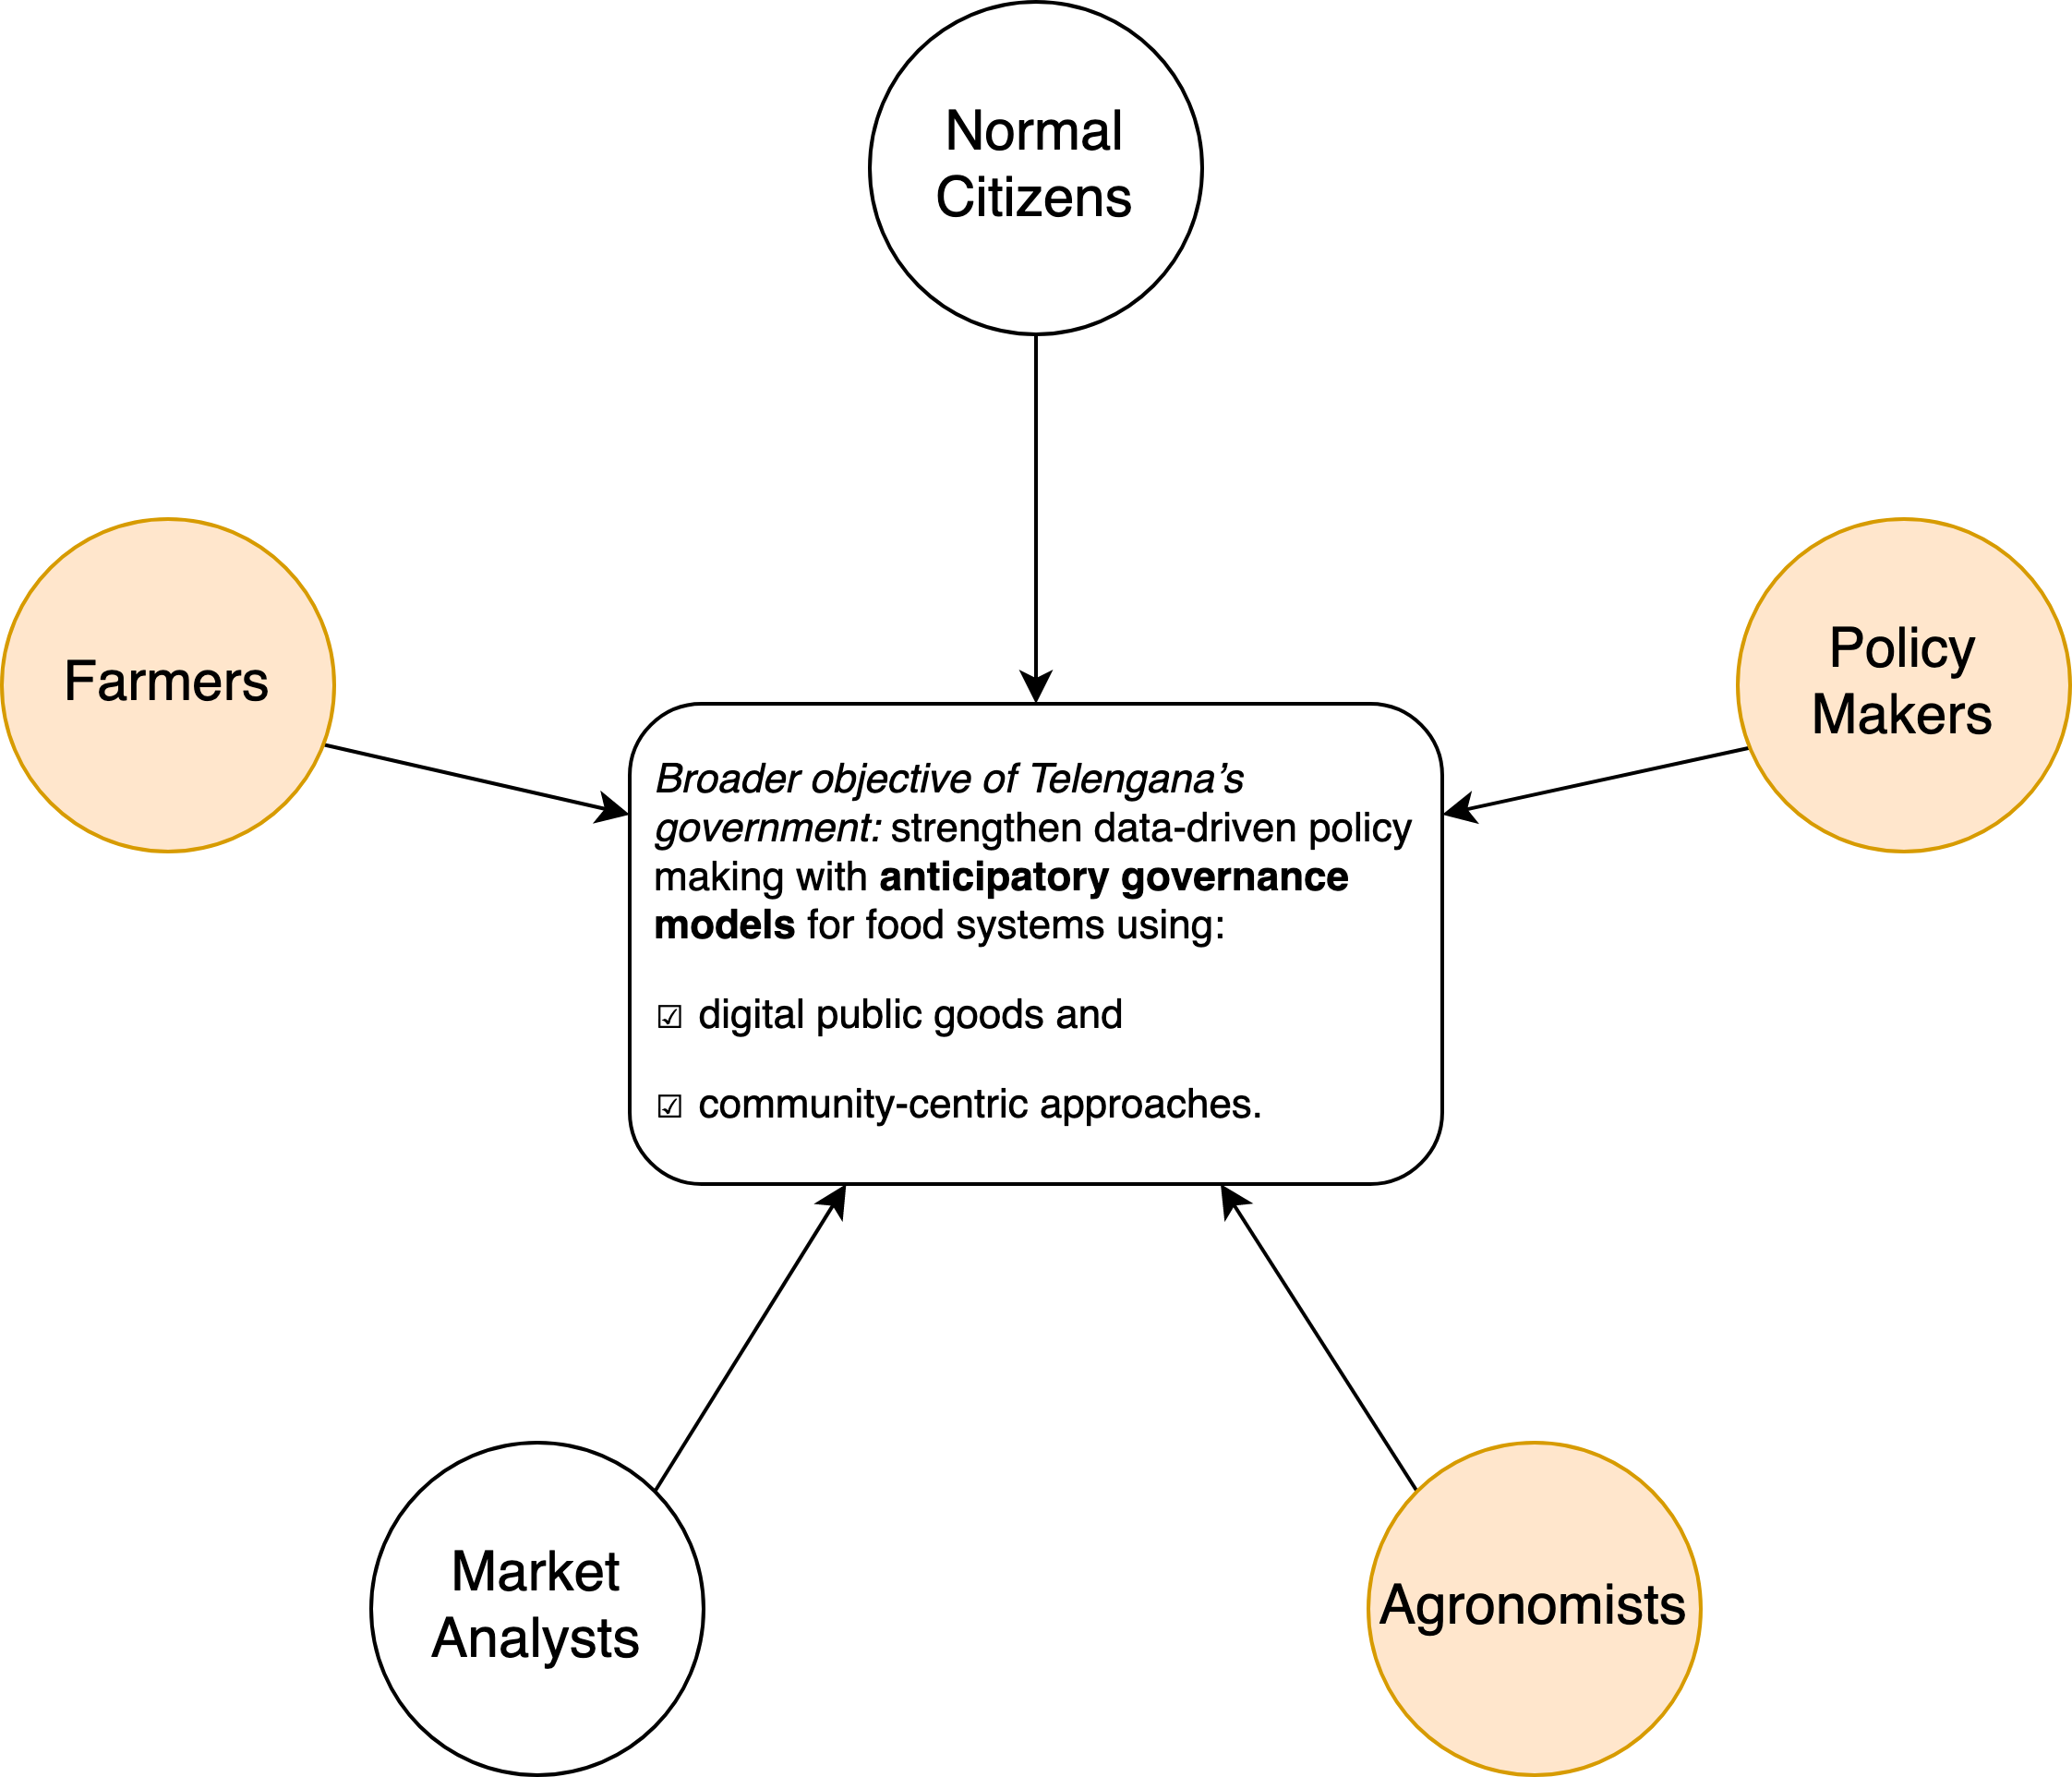
\includegraphics[scale=0.6]{../images_diagrams/stakeholders_in_broader_gov_objective.png}
\end{center}

%\smallskip\\
\end{flushleft}
%%%%%%%%%%%%%%%%%%%%%%%%%%%%%%%%%%%
%%%%%%%%%%%% THE GOALS %%%%%%%%%%%%
%%%%%%%%%%%%%%%%%%%%%%%%%%%%%%%%%%%
\subsubsection{Goals}
The following table lists an aggregate collection of the goals that serve the three main stakeholders that are in the scope of this system.

%%%% GOALS TABLE %%%%

\begin{center}
\renewcommand{\arraystretch}{1.25}
\begin{tabular}{|c| >{\raggedright\arraybackslash}p{12cm}|} \hline
    \textbf{ID} & \textbf{Goals}\\
    \hline
    G\addOne{goals_counter}  & Farmers can visualize relevant data and suggestions based on their location and type of production.\\ 
    \hline
    G\addOne{goals_counter}  & Agronomists and farmers can view weather forecast data.\\ 
    \hline
    G\addOne{goals_counter}  & Farmers can interact with others farmers and agronomists by requesting for help and suggestions.\\
    \hline
    G\addOne{goals_counter}  & Farmers can create discussion forums with other farmers.\\
    \hline
    G\addOne{goals_counter}  & Agronomists can supervise a sub-area inside the region. \\
    \hline
    G\addOne{goals_counter}  & Agronomists can view the ranking of farmers’ performance in their specific area.\\
    \hline
    G\addOne{goals_counter}  & Agronomists can visualize and update a daily plan to visit farms in their area.\\
    \hline
    G\addOne{goals_counter}  & Agronomists can specify the deviations from their daily plan and confirm the execution of their daily plan at the end of each day.\\
    \hline
    G\addOne{goals_counter}  & Telengana’s policy makers can view the performance of the farmers and the ranking of the farmers.\\
    \hline
    G\addOne{goals_counter} & Telengana’s policy makers can determine if support from agronomists and well-performing farmers produces significant results.\\
    \hline
\end{tabular}
\end{center}

%%%%%%%%%%%%%%%%%%%%%%%%%%%%%%%%%%%
%%%%%%%%%%%%% PHENOMENA %%%%%%%%%%%
%%%%%%%%%%%%%%%%%%%%%%%%%%%%%%%%%%%
\subsection{Scope}

\begin{flushleft} %Here we include an analysis of the world and of the shared phenomena 

Considering the three users in the scope of this initiative, the design of the system must first consider the following phenomena in context in which the system will operate.

%%%% PHENOMENA TABLE %%%%

\end{flushleft}
\begin{center}
\renewcommand{\arraystretch}{1.25}
\begin{tabular}{|>{\raggedright\arraybackslash}m{12cm}|c|} \hline
    \textbf{Phenomena} & \textbf{Type}\\ \hline % adds a line
    Lorem ipsum dolor sit amet, consectetuer adipiscing elit. & W \\
    \hline
    Ut purus elit, vestibulum ut, placerat ac, adipiscing vitae, felis. & M\\
    \hline
    Curabitur dictum gravidamauris. & S\\
    \hline
\end{tabular}
\end{center}

\subsection{Definitions, Acronyms, Abbreviations}

%%%% DEFINITIONS TABLE %%%%

\begin{center}
\renewcommand{\arraystretch}{1.25}
\begin{tabular}{l >{\raggedright\arraybackslash}m{12cm} } \hline
    \textbf{Term} & \textbf{Definition}\\ 
	Policy Maker & definition of policy maker \\
	Agronomist & definition of agronomist \\
    Farmer & A user who uses DREAM to help manage data relating to their farms and fields.\\
    Field & One enclosed area that corresponds to one crop. Many fields can make up a farm. The locations of the various fields do not need to be co-located.\\
    Farm & A set of one or many fields that are managed by one farmer.\\
    DREAM & The system described in this document; Data-dRiven PrEdictive FArMing\\
    Production yields & The amount of crop harvested compared to the amount of crop planted. Measured comparatively by percentage or numerically by weight.\\
    User & Farmer, agronomist, or policy user; anyone who uses the system.\\
    \hline
\end{tabular}
\end{center}



\subsection{Revision History}
\subsection{Reference Documents}
\subsection{Document Structure}